%
%
% UCSD Doctoral Dissertation Template
% -----------------------------------
% https://github.com/ucsd-thesis/ucsd-thesis
%
%
% ----------------------------------------------------------------------
% WARNING:
%
%   This template has not endorced by OGS or any other official entity.
%   The official formatting guide can be obtained from OGS.
%   It can be found on the web here:
%   http://grad.ucsd.edu/_files/academic-affairs/Dissertations_Theses_Formatting_Manual.pdf
%
%   No guaranty is made that this LaTeX class conforms to the official UCSD guidelines.
%   Make sure that you check the final document against the Formatting Manual.
%
%   That being said, this class has been routinely used for successful
%   publication of doctoral theses.
%
%   The ucsd.cls class files are only valid for doctoral dissertations.
%
%
% ----------------------------------------------------------------------
% GETTING STARTED:
%
%   Lots of information can be found on the project wiki:
%   http://code.google.com/p/ucsd-thesis/wiki/GettingStarted
%
%
%   To make a pdf from this template use the command:
%     pdflatex template
%
%
%   To get started please read the comments in this template file
%   and make changes as appropriate.
%
%   If you successfully submit a thesis with this package please let us
%   know.
%
%
% ----------------------------------------------------------------------
% KNOWN ISSUES:
%
%   Currently only the 12pt size conforms to the UCSD requirements.
%   The 10pt and 11pt options make the footnote fonts too small.
%
%
% ----------------------------------------------------------------------
% HELP/CONTACT:
%
%   If you need help try the ucsd-thesis google group:
%   http://groups.google.com/group/ucsd-thesis
%
%
% ----------------------------------------------------------------------
% BUGS:
%
%   Please report all bugs at:
%   https://github.com/ucsd-thesis/ucsd-thesis/issues
%
%
% ----------------------------------------------------------------------
% More control of the formatting of your thesis can be achieved through
% modifications of the included LaTeX class files:
%
%   * ucsd.cls    -- Class file
%   * uct10.clo   -- Configuration files for font sizes 10pt, 11pt, 12pt
%     uct11.clo
%     uct12.clo
%
% ----------------------------------------------------------------------



% Setup the documentclass
% default options: 12pt, oneside, final
%
% fonts: 10pt, 11pt, 12pt -- are valid for UCSD dissertations.
% sides: oneside, twoside -- note that two-sided theses are not accepted
%                            by OGS.
% mode: draft, final      -- draft mode switches to single spacing,
%                            removes hyperlinks, and places a black box
%                            at every overfull hbox (check these before
%                            submission).
% chapterheads            -- Include this if you want your chapters to read:
%                              Chapter 1
%                              Title of Chapter
%
%                            instead of
%                              1 Title of Chapter
\documentclass[12pt,chapterheads]{ucsd}



% Include all packages you need here.
% Some standard options are suggested below.
%
% See the project wiki for information on how to use
% these packages. Other useful packages are also listed there.
%
%   http://code.google.com/p/ucsd-thesis/wiki/GettingStarted



%% AMS PACKAGES - Chances are you will want some or all
%    of these if writing a dissertation that includes equations.
%  \usepackage{amsmath, amscd, amssymb, amsthm}

%% GRAPHICX - This is the standard package for
%    including graphics for latex/pdflatex.
\usepackage{scrextend}
\usepackage{pslatex}
\usepackage{graphicx}

%% CAPTION
% This overrides some of the ugliness in ucsd.cls and
% allows the text to be double-spaced while letting figures,
% tables, and footnotes to be single-spaced--all OGS requirements.
% NOTE: Must appear after graphics and ams math
\makeatletter
\gdef\@ptsize{2}% 12pt documents
\let\@currsize\normalsize
\makeatother
\usepackage{setspace}
\doublespace
\usepackage[font=small, width=0.9\textwidth]{caption}

%% SUBFIG - Use this to place multiple images in a
%    single figure.  Subfig will handle placement and
%    proper captioning (e.g. Figure 1.2(a))
% \usepackage{subfig}

%% TIMES FONT - replacements for Computer Modern
%%   This package will replace the default font with a
%%   Times-Roman font with math support.
% \usepackage[T1]{fontenc}
% \usepackage{mathptmx}

%% INDEX
%   Uncomment the following two lines to create an index:
% \usepackage{makeidx}
% \makeindex
%   You will need to uncomment the \printindex line near the
%   bibliography to display the index.  Use the command
% \index{keyword}
%   within the text to create an entry in the index for keyword.
%   To compile a LaTeX document with an index the 'makeindex'
%   command will need to be run.  See the wiki for more details.

%% HYPERLINKS
%   To create a PDF with hyperlinks, you need to include the hyperref package.
%   THIS HAS TO BE THE LAST PACKAGE INCLUDED!
%   Note that the options plainpages=false and pdfpagelabels exist
%   to fix indexing associated with having both (ii) and (2) as pages.
%   Also, all links must be black according to OGS.
%   See: http://www.tex.ac.uk/cgi-bin/texfaq2html?label=hyperdupdest
%   Note: This may not work correctly with all DVI viewers (i.e. Yap breaks).
%   NOTE: hyperref will NOT work in draft mode, as noted above.
% \usepackage[colorlinks=true, pdfstartview=FitV,
%             linkcolor=black, citecolor=black,
%             urlcolor=black, plainpages=false,
%             pdfpagelabels]{hyperref}
% \hypersetup{ pdfauthor = {Your Name Here},
%              pdftitle = {The Title of The Dissertation},
%              pdfkeywords = {Keywords for Searching},
%              pdfcreator = {pdfLaTeX with hyperref package},
%              pdfproducer = {pdfLaTeX} }
% \urlstyle{same}
% \usepackage{bookmark}


%% CITATIONS
% Sets citation format
% and fixes up citations madness
\usepackage{microtype}  % avoids citations that hang into the margin


%% FOOTNOTE-MAGIC
% Enables footnotes in tables, re-referencing the same footnote multiple times.
\usepackage{footnote}
\makesavenoteenv{tabular}
\makesavenoteenv{table}


%% TABLE FORMATTING MADNESS
% Enable all sorts of fun table tricks
\usepackage{rotating}  % Enables the sideways environment (NCPW)
\usepackage{array}  % Enables "m" tabular environment http://ctan.org/pkg/array
\usepackage{booktabs}  % Enables \toprule  http://ctan.org/pkg/array



\begin{document}

%% FRONT MATTER
%
%  All of the front matter.
%  This includes the title, degree, dedication, vita, abstract, etc..
%  Modify the file template_frontmatter.tex to change these pages.

\title{Making sense of microbial populations from representative samples}

\author{James T. Morton}
\degreeyear{2018}

% Master's Degree theses will NOT be formatted properly with this file.
\degreetitle{Doctor of Philosophy}

\field{Computer Science}

\chair{Professor Rob Knight}
% Uncomment the next line iff you have a Co-Chair
% \cochair{Professor Cochair Semimaster}
%
% Or, uncomment the next line iff you have two equal Co-Chairs.
%\cochairs{Professor Chair Masterish}{Professor Chair Masterish}

%  The rest of the committee members  must be alphabetized by last name.
\othermembers{
Professor Pieter Dorrestein\\
Professor Rachel Dutton\\
Professor Yoav Freund\\
Professor Siavash Mirarab
}
\numberofmembers{5} % |chair| + |cochair| + |othermembers|


%% START THE FRONTMATTER
%
\begin{frontmatter}

%% TITLE PAGES
%
%  This command generates the title, copyright, and signature pages.
%
\makefrontmatter

%% DEDICATION
%
%  You have three choices here:
%    1. Use the ``dedication'' environment.
%       Put in the text you want, and everything will be formated for
%       you. You'll get a perfectly respectable dedication page.
%
%
%    2. Use the ``mydedication'' environment.  If you don't like the
%       formatting of option 1, use this environment and format things
%       however you wish.
%
%    3. If you don't want a dedication, it's not required.
%
%
\begin{dedication}
  To my friends and family who paved the road and lit the journey.
\end{dedication}


% \begin{mydedication} % You are responsible for formatting here.
%   \vspace{1in}
%   \begin{flushleft}
% 	To me.
%   \end{flushleft}
%
%   \vspace{2in}
%   \begin{center}
% 	And you.
%   \end{center}
%
%   \vspace{2in}
%   \begin{flushright}
% 	Which equals us.
%   \end{flushright}
% \end{mydedication}



%% EPIGRAPH
%
%  The same choices that applied to the dedication apply here.
%
\begin{epigraph} % The style file will position the text for you.
  \emph{The `paradox' is only a conflict between reality and your feeling of what reality `ought to be'}\\
  ---Richard Feynman
\end{epigraph}

% \begin{myepigraph} % You position the text yourself.
%   \vfil
%   \begin{center}
%     {\bf Think! It ain't illegal yet.}
%
% 	\emph{---George Clinton}
%   \end{center}
% \end{myepigraph}


%% SETUP THE TABLE OF CONTENTS
%
\tableofcontents

%%
%% This block was needed to re-format the title of the glossary to match the
%% headings of the list of figures and list of tables.
%%
%% start hack:
\renewcommand{\glossarysection}[2][]{
\newpage
\noindent
\centerline{LIST OF ABBREVIATIONS}
\addcontentsline{toc}{chapter}{List of Abbreviations}
}
%% end hack
\printglossary[title=List of Abbreviations,toctitle=List of Abbreviations,nonumberlist ]

\listoffigures  % Comment if you don't have any figures
\listoftables   % Comment if you don't have any tables


%% ACKNOWLEDGEMENTS
%
%  While technically optional, you probably have someone to thank.
%  Also, a paragraph acknowledging all coauthors and publishers (if
%  you have any) is required in the acknowledgements page and as the
%  last paragraph of text at the end of each respective chapter. See
%  the OGS Formatting Manual for more information.
%
\begin{acknowledgements}
  First, I would like to acknowledge Rob Knight, for his guidance that enabled me to
  grow as a person as well as a scientist.  This work was largely enabled by him and
  I am greatly thankful for his support.

  I would like to thank my committee members Pieter Dorrestein, Yoav Freund,
  Siavash Mirarab and Rachel Dutton not only for providing feedback for this
  thesis, but also for fostering years of collaborative science.

  This work couldn't have been done with out the strong support of the members of the
  Knight lab. Many thanks to the individuals responsible for the finances, logistics,
  and computational hardware maintainence that ultimately facilitated the sharing
  of ideas across public venues, namely Ulla Westerman, Jerry Kennedy, Gail Ackermann,
  Jeff DeReus, Michiko Souza, and Sarah Adams.  I would also like to acknowledge the
  multiple individuals that served as mentors, namely Jon Sanders, Daniel McDonald,
  Antonio Gonzalez, Yoshiki Vazquez-baeza, Zhenjiang Xu, Amnon Amir, Albert Barberán,
  Luke Thompson, Justine Debelius, Sejin Song, Jessica Metcalf, Greg Humphrey and Rob Quinn.
  My fellow peers brought the excitment into the lab, making my PhD experience
  thoroughly enjoyable, in particular Lisa Marotz, Qiyun Zhu, Stefan Janssen, Georg Loss,
  Anupriya Tripathi, Alison Vrbanac, Serene Lingjing Jiang, Antony Pearson,
  Peter Edge, Benjamin Pullman, Mingxun Wang, Richardo Silva, Alexander Aksenov,
  Louis-Felix Nothias-Scaglia and Brooke Anderson. Among the many collaborators,
  colleagues and mentors outside of UCSD responsible for contributing to
  this body of work, I would especially like to acknowledge Anna Edlund, Alex Washburne,
  Justin Silverman, John Karro, Iddo Friedberg, Manuel Lladser, Christopher Lowry,
  Noah Fierer, Benjamin Langmead, Jeff Leek and Susan Holmes for their
  thought-provoking insights.

  Finally, I would like to thank my friends and family for their love and support.
  In particular, my parents Jade and John Morton for their drive and care early
  on distilling my love in engineering, mathematics and science.  Rachael Morton
  for being a loveable sister and an angel on my shoulder.  And Juer
  Song, who is my pillar, my pillow and my greatest companion.

  Chapter 1, in full, is a reprint of the material as it appears in
  ``Methods for phylogenetic analysis of microbiome data''
  Alex D. Washburne, James T. Morton, Jon Sanders, Daniel McDonald,
  Qiyun Zhu, Angela M. Oliverio, Rob Knight  \emph{Nature Microbiology} 3, 2018. The dissertation author was the primary investigator and co-first author of this paper.

  Chapter 2, in full, is a reprint of the material as it appears in
  ``Uncovering the Horseshoe Effect in Microbial Analyses''
  James T. Morton, Liam Toran, Anna Edlund, Jessica L. Metcalf,
  Christian Lauber, Rob Knight \emph{mSystems}, 2, 2017.  The dissertation author was the primary investigator and first author of this paper.

  Chapter 3, in full, is a reprint of the material as it appears in
  ``Balance Trees Reveal Microbial Niche Differentiation''
  James T. Morton, Jon Sanders, Robert A. Quinn, Daniel McDonald, Antonio Gonzalez,
  Yoshiki Vázquez-Baeza, Jose A. Navas-Molina, Se Jin Song, Jessica L. Metcalf,
  Embriette R. Hyde, Manuel Lladser, Pieter C. Dorrestein, Rob Knight
  \emph{mSystems}, 2, 2017.  The dissertation author was the primary investigator and first author of this paper.

  Chapter 4 has been submitted for publication of the material as it may appear in
  Nature Biotechnology, 2019 ``Establishing microbial measurement standards with reference frames''
  James T. Morton,  Clarisse Marotz, Justin Silverman, Alex Washburne, Livia S. Zaramela,
  Anna Edlund, Karsten Zengler, Rob Knight. The dissertation author was the primary investigator and first author of this paper.


\end{acknowledgements}


%% VITA
%
%  A brief vita is required in a doctoral thesis. See the OGS
%  Formatting Manual for more information.
%
\begin{vitapage}
\begin{vita}

  \item[2014] B.~S. in Computer Science \emph{cum laude}, Miami University, OH
  \item[2014] B.~S. in Mathematics and Statistics \emph{cum laude}, Miami University, OH
  \item[2014] B.~S. in Electrical Engineering \emph{cum laude}, Miami University, OH
  \item[2014] B.~S. in Engineering Physics \emph{cum laude}, Miami University, OH
  \item[2018] Ph.~D. in Computer Science, University of California San Diego
\end{vita}
\begin{publications}
    \item \textsl{Author names marked with $\dagger$ indicate shared first co-authorship}.

    \item $\dagger$Alex D. Washburne, \textbf{$\dagger$James T. Morton}, Jon Sanders, Daniel McDonald, Qiyun Zhu, Angela M. Oliverio, Rob Knight  ``Methods for phylogenetic analysis of microbiome data'' \emph{Nature Microbiology} 3, 2018

    \item  \textbf{James T. Morton}, Liam Toran, Anna Edlund, Jessica L. Metcalf, Christian Lauber, Rob Knight ``Uncovering the Horseshoe Effect in Microbial Analyses'' \emph{mSystems}, 2, 2017

    \item \textbf{James T. Morton}, Jon Sanders, Robert A. Quinn, Daniel McDonald, Antonio Gonzalez, Yoshiki Vázquez-Baeza, Jose A. Navas-Molina, Se Jin Song, Jessica L. Metcalf, Embriette R. Hyde, Manuel Lladser, Pieter C. Dorrestein, Rob Knight ``Balance Trees Reveal Microbial Niche Differentiation'' \emph{mSystems}, 2, 2017

    \textsl{The following publications were not included as part of this dissertation, but were also significant byproducts of my doctoral training.}
\item  Stefan O Reber, Philip H  Siebler, Nina C  Donner, \textbf{James T Morton}, David G  Smith, Jared M  Kopelman, Kenneth R  Lowe, Kristen J  Wheeler, James H  Fox, James E  Hassell,  ``Immunization with a heat-killed preparation of the environmental bacterium Mycobacterium vaccae promotes stress resilience in mice'' \emph{Proceedings of the National Academy of Sciences}, 113, 2016

    \item  Jack A Gilbert, Robert A  Quinn, Justine  Debelius, Zhenjiang Z  Xu, James  Morton, Neha  Garg, Janet K  Jansson, Pieter C  Dorrestein, Rob  Knight,  ``Microbiome-wide association studies link dynamic microbial consortia to disease'' \emph{Nature}, 535, 2016

    \item  Yoshiki Vázquez-Baeza, Antonio  Gonzalez, Larry  Smarr, Daniel  McDonald, \textbf{James T Morton}, Jose A  Navas-Molina, Rob  Knight,  ``Bringing the dynamic microbiome to life with animations'' \emph{Cell host \& microbe}, 21, 2017


    \item  Albert Barberán, Robert R  Dunn, Brian J  Reich, Krishna  Pacifici, Eric B  Laber, Holly L  Menninger, \textbf{James T Morton}, Jessica B  Henley, Jonathan W  Leff, Shelly L  Miller,  ``The ecology of microscopic life in household dust'' \emph{Proc. R. Soc. B}, 282, 2015

    \item  Erin M Hill‐Burns, Justine W  Debelius, \textbf{James T Morton}, William T  Wissemann, Matthew R  Lewis, Zachary D  Wallen, Shyamal D  Peddada, Stewart A  Factor, Eric  Molho, Cyrus P  Zabetian,  ``Parkinson's disease and Parkinson's disease medications have distinct signatures of the gut microbiome'' \emph{Movement disorders}, 32, 2017


    \item  Amnon Amir, Daniel  McDonald, Jose A  Navas-Molina, Justine  Debelius, \textbf{James T Morton}, Embriette  Hyde, Adam  Robbins-Pianka, Rob  Knight,  ``Correcting for microbial blooms in fecal samples during room-temperature shipping'' \emph{MSystems}, 2, 2017

    \item  Amnon Amir, Daniel  McDonald, Jose A  Navas-Molina, Evguenia  Kopylova, \textbf{James T Morton}, Zhenjiang Zech  Xu, Eric P  Kightley, Luke R  Thompson, Embriette R  Hyde, Antonio  Gonzalez,  ``Deblur rapidly resolves single-nucleotide community sequence patterns'' \emph{MSystems}, 2, 2017

    \item  Alison Vrbanac, Justine W  Debelius, Lingjing  Jiang, \textbf{James T Morton}, Pieter  Dorrestein, Rob  Knight,  ``An Elegan (t) Screen for Drug-Microbe Interactions'' \emph{Cell host \& microbe}, 21, 2017

    \item  Sian MJ Hemmings, Stefanie  Malan-Müller, Leigh L  van den Heuvel, Brittany A  Demmitt, Maggie A  Stanislawski, David G  Smith, Adam D  Bohr, Christopher E  Stamper, Embriette R  Hyde, \textbf{James T Morton},  ``The microbiome in posttraumatic stress disorder and trauma-exposed controls: an exploratory study'' \emph{Psychosomatic medicine}, 79, 2017

    \item  Laura-Isobel McCall, \textbf{James T Morton}, Jean A  Bernatchez, Jair Lage  de Siqueira-Neto, Rob  Knight, Pieter C  Dorrestein, James H  McKerrow,  ``Mass spectrometry-based chemical cartography of a cardiac parasitic infection'' \emph{Analytical chemistry}, 89, 2017

    \item  Yoshiki Vázquez-Baeza, Chris  Callewaert, Justine  Debelius, Embriette  Hyde, Clarisse  Marotz, \textbf{James T Morton}, Austin  Swafford, Alison  Vrbanac, Pieter C  Dorrestein, Rob  Knight,  ``Impacts of the human gut microbiome on therapeutics'' \emph{Annual review of pharmacology and toxicology}, 58, 2018

    \item  Jessica L Metcalf, Se Jin  Song, \textbf{James T Morton}, Sophie  Weiss, Andaine  Seguin-Orlando, Frédéric  Joly, Claudia  Feh, Pierre  Taberlet, Eric  Coissac, Amnon  Amir,  ``Evaluating the impact of domestication and captivity on the horse gut microbiome'' \emph{Scientific reports}, 7, 2017

    \item  Lingjing Jiang, Amnon  Amir, \textbf{James T Morton}, Ruth  Heller, Ery  Arias-Castro, Rob  Knight,  ``Discrete false-discovery rate improves identification of differentially abundant microbes'' \emph{MSystems}, 2, 2017

    \item  Clifford A Kapono, \textbf{James T Morton}, Amina  Bouslimani, Alexey V  Melnik, Kayla  Orlinsky, Tal Luzzatto  Knaan, Neha  Garg, Yoshiki  Vázquez-Baeza, Ivan  Protsyuk, Stefan  Janssen,  ``Creating a 3D microbial and chemical snapshot of a human habitat'' \emph{Scientific reports}, 8, 2018

    \item  Daniel McDonald, Embriette  Hyde, Justine W  Debelius, \textbf{James T Morton}, Antonio  Gonzalez, Gail  Ackermann, Alexander A  Aksenov, Bahar  Behsaz, Caitriona  Brennan, Yingfeng  Chen,  ``American Gut: an Open Platform for Citizen Science Microbiome Research'' \emph{mSystems}, 3, 2018


    \item  Robert A Quinn, William  Comstock, Tianyu  Zhang, \textbf{James T Morton}, Ricardo  da Silva, Alda  Tran, Alexander  Aksenov, Louis-Felix  Nothias, Daniel  Wangpraseurt, Alexey V  Melnik,  ``Niche partitioning of a pathogenic microbiome driven by chemical gradients'' \emph{Science advances}, 4, 2018
\end{publications}
\end{vitapage}


%% ABSTRACT
%
%  Doctoral dissertation abstracts should not exceed 350 words.
%   The abstract may continue to a second page if necessary.
%
\begin{abstract}
Microbiomes make up the vast majority of life on Earth, and we are just beginning to understand how to
study them using high-throughput omics.  However, analysis of microbial populations is complicated by
numerous statistical challenges.  We first outline these challenges in the context of phylogenetically
aware methods, then focus on two concepts: the horseshoe effect and compositionality.

The horseshoe effect is a phenomenon that can lead to horseshoe patterns appearing in low dimensional
representations of high dimensional data.  For multiple decades, this pattern confounded ecologists
when studying populations across multiple environmental conditions.  Here, we show that the
horseshoe effect arises from distance saturation, and can indicative of microbial population
displacement. This phenomenon is illustrated across a soil study and a
decomposition study.

In the second part of the thesis, we will discuss identifiability due to representative sampling,
also known as compositionality. Statistical laws have shown that it's possible to obtain
unbiased estimators for population proportions from representative samples.
However, based on representative samples alone, it is not possible to determine which species abundances
have grown or declined, since there is an infinite number of outcomes that can explain
the same change in proportions. In the biological sciences, this problem is also known as the
differential abundance problem, which is critical for determining which microbes have been altered across
experimental outcomes. Here, we show that in order to estimate which species have been altered,
the total population size needs to be estimated.

We present two workarounds to this problem that ultimately negating the need to estimate total
population size. The first solution is using ratios, analogous to concentrations in chemistry.
We will showcase the usefulness of this technique on a soils study and a cystic fibrosis study.
The second solution is using ranks as a proxy to feature importances. Rather than attempting to
compute absolute change, we can compute relative change, ultimately ranking which microbes have
increased or decreased the most across different experimental conditions.
We show how these ranks can be computed using multinomial regression and can
facilitate reproducible findings in the context of oral microbial communities and atopic dermatitis.
\end{abstract}


\end{frontmatter}






%% DISSERTATION

% A common strategy here is to include files for each of the chapters. I.e.,
% Place the chapters is separate files:
%   chapter1.tex, chapter2.tex
% Then use the commands:
%   \include{chapter1}
%   \include{chapter2}
%
% Of course, if you prefer, you can just start with
%   \chapter{My First Chapter Name}
% and start typing away.
\chapter{Just a Test}
This is only a test.
\section{A section}
Lorem ipsum dolor sit amet, consectetuer adipiscing elit. Nulla odio
sem, bibendum ut, aliquam ac, facilisis id, tellus. Nam posuere pede
sit amet ipsum. Etiam dolor. In sodales eros quis pede.  Quisque sed
nulla et ligula vulputate lacinia. In venenatis, ligula id semper
feugiat, ligula odio adipiscing libero, eget mollis nunc erat id orci.
Nullam ante dolor, rutrum eget, vestibulum euismod, pulvinar at, nibh.
In sapien. Quisque ut arcu. Suspendisse potenti. Cras consequat cursus
nulla.

\subsection{A Figure Example}
\label{ssec:figure_example}

This subsection shows a sample figure.

\begin{figure}[h]
  \centering
  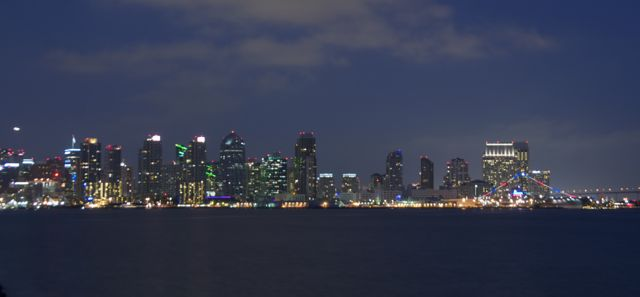
\includegraphics[width=0.5\textwidth]{sandiego}
  \caption[A picture of San Diego. Short figure caption must be \protect{$< 4$} lines in the list of figures]
{A picture of San Diego.  Short figure caption must be \protect{$< 4$} lines in the list of figures and match the start of the main figure caption verbatim. Note that figures must be on their own line (no neighboring text) and captions must be single-spaced and appear \protect\textit{below} the figure.  Captions can be as long as you want, but if they are longer than 4 lines in the list of figures, you must provide a short figure caption.\index{SanDiego}}
  \label{fig:sandiego}
\end{figure}

\subsection{A Table Example}

While in Section \ref{ssec:figure_example} Figure \ref{fig:sandiego} we had a majestic figure, here we provide a crazy table example.


%%%% TABLE 1 %%%%
\vspace{0.25in}
\begin{table}[!ht]
\caption[A table of when I get hungry.  Short table caption must be \protect{$< 4$} lines in the list of tables]{A table of when I get hungry. Short table caption must be \protect{$< 4$} lines in the list of tables and match the start of the main table caption verbatim.  Note that tables must be on their own line (no neighboring text) and captions must be single-spaced and appear \protect\textit{above} the table.  Captions can be as long as you want, but if they are longer than 4 lines in the list of figures, you must provide a short figure caption.}

\vspace{-0.25in}
\begin{center}
\begin{tabular}{|p{1in}|p{2in}|p{3in}|}

\hline
Time of day & Hunger Level & Preferred Food \\

\hline
8am & high & IHOP (French Toast) \\

\hline
noon & medium & Croutons (Tomato Basil Soup \& Granny Smith Chicken Salad) \\

\hline
5pm & high & Bombay Coast (Saag Paneer) or Hi Thai (Pad See Ew) \\

\hline
8pm & medium & Yogurt World (froyo!) \\

\hline
\end{tabular}
\end{center}
\label{tab:analysis3}
\end{table}



%% APPENDIX
\appendix
\chapter{Final notes}
What to do about things \cite{Martin_1983}.  What did he say \cite{Rilling_Insel_1999}.
  Remove me in case of abdominal pain.



%% END MATTER
% \printindex %% Uncomment to display the index
% \nocite{}  %% Put any references that you want to include in the bib
%               but haven't cited in the braces.
\bibliographystyle{alpha}  %% This is just my personal favorite style.
%                              There are many others.
%\setlength{\bibleftmargin}{0.25in}  % indent each item
%\setlength{\bibindent}{-\bibleftmargin}  % unindent the first line
%\def\baselinestretch{1.0}  % force single spacing
%\setlength{\bibitemsep}{0.16in}  % add extra space between items
\bibliography{template}  %% This looks for the bibliography in template.bib
%                          which should be formatted as a bibtex file.
%                          and needs to be separately compiled into a bbl file.
\end{document}

